%%%%%%%%%%%%%%%%%%%%%%%%%%%%%%%%%%%%%%%%%
% Arsclassica Article
% LaTeX Template
% Version 1.1 (1/8/17)
%
% This template has been downloaded from:
% http://www.LaTeXTemplates.com
%
% Original author:
% Lorenzo Pantieri (http://www.lorenzopantieri.net) with extensive modifications by:
% Vel (vel@latextemplates.com)
%
% License:
% CC BY-NC-SA 3.0 (http://creativecommons.org/licenses/by-nc-sa/3.0/)
%
%%%%%%%%%%%%%%%%%%%%%%%%%%%%%%%%%%%%%%%%%

%----------------------------------------------------------------------------------------
%	PACKAGES AND OTHER DOCUMENT CONFIGURATIONS
%----------------------------------------------------------------------------------------

\documentclass[
10pt, % Main document font size
a4paper, % Paper type, use 'letterpaper' for US Letter paper
oneside, % One page layout (no page indentation)
%twoside, % Two page layout (page indentation for binding and different headers)
headinclude,footinclude, % Extra spacing for the header and footer
BCOR5mm, % Binding correction
]{scrartcl}


\usepackage{longtable}
\usepackage{array}
\usepackage{pdfpages}
\usepackage{booktabs}
\usepackage{mdwlist}

\usepackage[dvipsnames]{xcolor}
\usepackage{colortbl}

\newcommand{\abr}[1]{\textsc{#1}}

\newcommand{\name}{The Bachelor of Science in Artificial Intelligence}
\newcommand{\short}{\abr{bsai}}
\newcommand{\ai}{\abr{ai}}
\newcommand{\aim}{\abr{aim}}

\newcommand{\question}[1]{\noindent \textbf{#1}}
\newcommand{\answer}[1]{\textit{#1}}

\newcommand{\bscourse}[1]{\abr{aibs} \hyperref[aibs:#1]{#1}}
\newcommand{\bacourse}[2]{\abr{aiba} \hyperref[aiba:#1]{#1}}
%%%%%%%%%%%%%%%%%%%%%%%%%%%%%%%%%%%%%%%%%
% Arsclassica Article
% Structure Specification File
%
% This file has been downloaded from:
% http://www.LaTeXTemplates.com
%
% Original author:
% Lorenzo Pantieri (http://www.lorenzopantieri.net) with extensive modifications by:
% Vel (vel@latextemplates.com)
%
% License:
% CC BY-NC-SA 3.0 (http://creativecommons.org/licenses/by-nc-sa/3.0/)
%
%%%%%%%%%%%%%%%%%%%%%%%%%%%%%%%%%%%%%%%%%

%----------------------------------------------------------------------------------------
%	REQUIRED PACKAGES
%----------------------------------------------------------------------------------------

\usepackage[
nochapters, % Turn off chapters since this is an article        
beramono, % Use the Bera Mono font for monospaced text (\texttt)
eulermath,% Use the Euler font for mathematics
pdfspacing, % Makes use of pdftex’ letter spacing capabilities via the microtype package
dottedtoc % Dotted lines leading to the page numbers in the table of contents
]{style/classicthesis} % The layout is based on the Classic Thesis style

\usepackage{style/arsclassica} % Modifies the Classic Thesis package

\usepackage[T1]{fontenc} % Use 8-bit encoding that has 256 glyphs

\usepackage[utf8]{inputenc} % Required for including letters with accents

\usepackage{graphicx} % Required for including images
\graphicspath{{Figures/}} % Set the default folder for images

\usepackage{enumitem} % Required for manipulating the whitespace between and within lists

\usepackage{lipsum} % Used for inserting dummy 'Lorem ipsum' text into the template

\usepackage{subfig} % Required for creating figures with multiple parts (subfigures)

\usepackage{amsmath,amssymb,amsthm} % For including math equations, theorems, symbols, etc

\usepackage{varioref} % More descriptive referencing

%----------------------------------------------------------------------------------------
%	THEOREM STYLES
%---------------------------------------------------------------------------------------

\theoremstyle{definition} % Define theorem styles here based on the definition style (used for definitions and examples)
\newtheorem{definition}{Definition}

\theoremstyle{plain} % Define theorem styles here based on the plain style (used for theorems, lemmas, propositions)
\newtheorem{theorem}{Theorem}

\theoremstyle{remark} % Define theorem styles here based on the remark style (used for remarks and notes)

%----------------------------------------------------------------------------------------
%	HYPERLINKS
%---------------------------------------------------------------------------------------

\hypersetup{
%draft, % Uncomment to remove all links (useful for printing in black and white)
colorlinks=true, breaklinks=true, bookmarks=true,bookmarksnumbered,
urlcolor=webbrown, linkcolor=RoyalBlue, citecolor=webgreen, % Link colors
pdftitle={}, % PDF title
pdfauthor={\textcopyright}, % PDF Author
pdfsubject={}, % PDF Subject
pdfkeywords={}, % PDF Keywords
pdfcreator={pdfLaTeX}, % PDF Creator
pdfproducer={LaTeX with hyperref and ClassicThesis} % PDF producer
} % Include the structure.tex file which specified the document structure and layout

\hyphenation{Fortran hy-phen-ation} % Specify custom hyphenation points in words with dashes where you would like hyphenation to occur, or alternatively, don't put any dashes in a word to stop hyphenation altogether

%----------------------------------------------------------------------------------------
%	TITLE AND AUTHOR(S)
%----------------------------------------------------------------------------------------

\title{\normalfont\spacedallcaps{BS in AI Proposal}} % The article title

%\subtitle{Subtitle} % Uncomment to display a subtitle

%\author{\spacedlowsmallcaps{John Smith* \& James Smith\textsuperscript{1}}} % The article author(s) - author affiliations need to be specified in the AUTHOR AFFILIATIONS block

\date{} % An optional date to appear under the author(s)

%----------------------------------------------------------------------------------------

\begin{document}

%----------------------------------------------------------------------------------------
%	HEADERS
%----------------------------------------------------------------------------------------

\renewcommand{\sectionmark}[1]{\markright{\spacedlowsmallcaps{#1}}} % The header for all pages (oneside) or for even pages (twoside)
%\renewcommand{\subsectionmark}[1]{\markright{\thesubsection~#1}} % Uncomment when using the twoside option - this modifies the header on odd pages
\lehead{\mbox{\llap{\small\thepage\kern1em\color{halfgray} \vline}\color{halfgray}\hspace{0.5em}\rightmark\hfil}} % The header style

\pagestyle{scrheadings} % Enable the headers specified in this block

%----------------------------------------------------------------------------------------
%	TABLE OF CONTENTS & LISTS OF FIGURES AND TABLES
%----------------------------------------------------------------------------------------

\maketitle % Print the title/author/date block

\setcounter{tocdepth}{2} % Set the depth of the table of contents to show sections and subsections only

\tableofcontents % Print the table of contents

%\listoftables % Print the list of tables

% \let\thefootnote\relax\footnotetext{* \textit{Department of Biology, University of Examples, London, United Kingdom}}

% \let\thefootnote\relax\footnotetext{\textsuperscript{1} \textit{Department of Chemistry, University of Examples, London, United Kingdom}}

%----------------------------------------------------------------------------------------


%----------------------------------------------------------------------------------------
%	INTRODUCTION
%----------------------------------------------------------------------------------------

\section{Description}

Artificial Intelligence is the study of creating computer systems that
learn from data an interactions to create systems that can reason,
generate text and images, and interact in ways that resemble humans.
%
\name{} (\short{}) is a highly technical program the trains
students to build new \ai{} tools from the ground up, understand the
training of models from both a data and systems perspective, and then
use those techniques in interdisciplinary applications.
%
The first two years of the program develop a strong technical
foundation in programming and understanding the theory of statistical
learning, symbolic reasoning, and optimization.
%
The following two years focuses on deploying those techniques in
interdisciplinary applications to enable students to be able to not
just build state-of-the-art \ai{} systems but to also think critically
about the effective, ethical application of \ai{}.

\section{Requirements}

\begin{figure}

  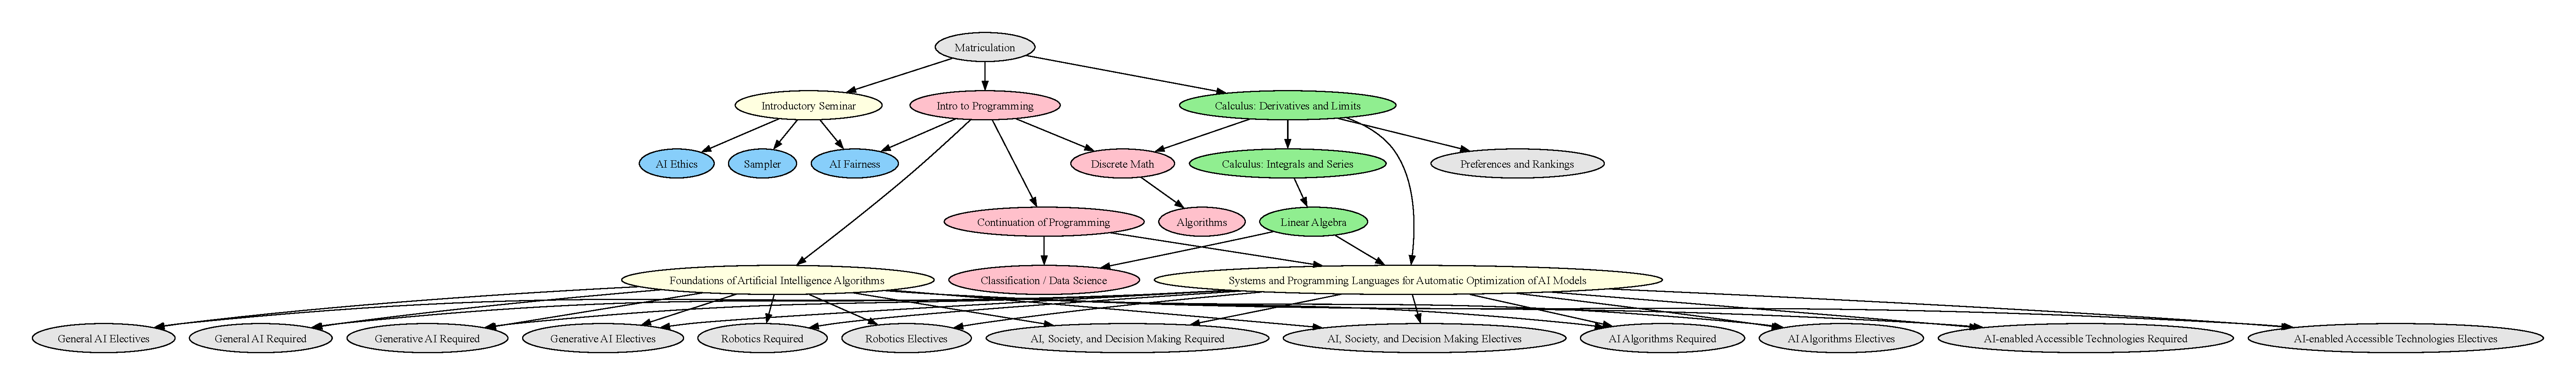
\includegraphics[width=1.0\linewidth]{dependency_graph/all}
  \caption{Dependency graph of the program topics.}
\end{figure}

\section{Learning Outcomes}

% \begin{itemize}
%     \item \textbf{Foundational Knowledge}
%     \begin{itemize}
%         \item Understand and apply core principles of Artificial Intelligence, including classical algorithms, neural networks, and modern machine learning techniques.
%         \item Develop a strong grounding in computational complexity, data structures, and efficient algorithms for large-scale data analysis.
%     \end{itemize}

%     \item \textbf{Technical Proficiency}
%     \begin{itemize}
%         \item Design, implement, and optimize \ai{} systems for specific real-world applications in areas such as creativity, food systems, law, and fairness.
%         \item Utilize object-oriented programming and advanced data handling techniques to build scalable and efficient \ai{} solutions.
%     \end{itemize}

%     \item \textbf{Interdisciplinary Integration}
%     \begin{itemize}
%         \item Apply insights from ethics, philosophy, and social sciences to the design and evaluation of \ai{} systems.
%         \item Explore interdisciplinary applications of \ai{} to address societal challenges.
%     \end{itemize}

%     \item \textbf{Ethical and Societal Impact}
%     \begin{itemize}
%         \item Identify and analyze the ethical implications of \ai{} technologies, including issues of algorithmic bias, decision-making opacity, and autonomous system deployment.
%         \item Develop strategies to mitigate potential harm and ensure fairness, inclusivity, and accountability in \ai{} systems.
%     \end{itemize}

%     \item \textbf{Critical Thinking and Problem Solving}
%     \begin{itemize}
%         \item Use formal reasoning, evaluations, and evaluative models to evaluate and improve \ai{} systems.
%         \item Critically assess \ai{} tools and outputs to ensure reliability, efficiency, and alignment with intended goals.
%     \end{itemize}

%     \item \textbf{Communication and Collaboration}
%     \begin{itemize}
%         \item Articulate complex \ai{} concepts and their implications to technical and non-technical audiences.
%         \item Collaborate effectively in multidisciplinary teams to design \ai{} solutions that address diverse perspectives and priorities.
%     \end{itemize}
% \end{itemize} 


\begin{itemize}
        \item Understand and apply core principles of modern and classic AI.

        \item Design and build efficient, scalable and effective algorithms and systems for real-world applications.

        \item Configure, train and deploy existing models for real-world applications.

        \item Critically assess ai tools and outputs to ensure reliability, efficiency, safety and alignment with intended goals.

        \item Apply insights from ethics and social sciences to interdisciplinary applications of \ai{} to address societal challenges and risks of AI such as bias, transparency, fairness and accountability. 

        \item Collaborate and communicate effectively in multidisciplinary teams to design AI solutions that address diverse perspectives and priorities.
\end{itemize} 

\section{Relationships}


\subsection{Relationship to AIM}

In Spring 2024, UMD launched the Artificial Intelligence Interdisciplinary Institute at Maryland (AIM), bringing together AI experts across campus to focus on responsible, ethical development and use of the technology to advance public good in industry, government and society. Given the rapid pace of AI development, a core part of AIM’s mission is to reimagine learning in the face of these drastic changes through the introduction of four new interdisciplinary programs, including Bachelor of Science and Bachelor of Arts degrees in Artificial Intelligence. Students across all majors will learn the principles of AI and how they apply to their field of study.

As part of this initiative, \short{} is designed to be an interdisciplinary program from the
ground up and thus will use faculty with joint appointments with
\aim{} and homes for courses to create the new interdisciplinary
courses required for this program.


\subsection{Relationship to Computer Science}

This section outlines how \short{} would be different from the existing computer science degree (with which is shares multiple courses).  The first, consistent with its inclusion in \aim{} is that it's interdisciplinary.  Second, it offers an introduction to \abr{ai} early in students' curriculum.  Finally, it offers another option to help cope with the large demand for computational majors at the University of Maryland.

\paragraph{Interdisciplinary}

At present, the computer science degree (where most students learn the foundations of artificial intelligence) while highly technical, does not require courses in ethics, social issues, or in the foundation of intelligence.
%
Because Maryland is a world leader in these areas and because \abr{ai}'s broad impact on society, future leaders in \abr{ai} will need these softer skills to build effective systems that will benefit society.

Moreover, the interdisciplinary courses offered by \short{} will serve as opportunities to bolster the interdisciplinary research that is a fundamental goal of \aim{}: the coursework and projects that begin in this program can lead to startups, research projects, and synergies across the campus.

\paragraph{Early Onramp}

While there is already an machine learning \abr{ml} concentration within the computer science degree, \abr{ai} courses are locked behind long prerequisite chains (the first course in the current \abr{ml} degree is CMSC 320, and the other \abr{ai}-relevant courses are all 400 level).  
%
By integrating \abr{ai} concepts earlier in the curriculum (starting in the introductory seminar and programming courses), students will be able to see the relevance of \abr{ai} to their interdisciplinary interests.

\paragraph{Complementing Existing Computational Majors}

There is a large demand for computational majors at the University of Maryland.  
%
While computer science and information studies are the largest, there are multiple others.
%
Given the pervasiveness of \abr{ai}, this offers another route: one that offers a rigorous technical component with interdisciplinary connections.\footnote{Of course, there are motivated students that create their own programs that are interdisciplinary (e.g., by double majoring or selecting a minor).  By formalizing these processes, we will both make it easier for more students to build this interdisciplinary path and provide students credentials.}
%
The goal is that having an alternate route will be able to attract students from diverse backgrounds and prepare them for jobs in \abr{ai}. 




\section{Requirements}

  
%%%%%%%%%%%%%%%%%%%%%%%%%%%%%%%%%%%%%%%%%%%%%%%%%%%%%%
% DO NOT EDIT THIS FILE, IT IS AUTOMATICALLY GENERATED
% INSTEAD, EDIT THE FILE HERE:
%
% https://docs.google.com/spreadsheets/d/1qRaEKxhyfwjHDWa3burGeqK0zeC00Br8NhJfnMWXJdk/edit?usp=sharing
%
% If you edit this file, your changes will be overwritten from this
% spreadsheet linked above.
%%%%%%%%%%%%%%%%%%%%%%%%%%%%%%%%%%%%%%%%%%%%%%%%%%%%%%%
\rowcolors{2}{gray!25}{white}
\begin{longtable}{p{7cm}>{\raggedleft\arraybackslash}p{7cm}}
Topic & Courses \\
\toprule
\textbf{Single Variable Calculus} [4 Credits] & MATH~340 or MATH~140       \\
\textbf{Introductory Seminar} [1 Credits] & AI~101                         \\
\textbf{Intro to Programming} [4 Credits] & CMSC~141, CMSC~131, or INST~326 \\
\textbf{AI's Ethical Frontiers} [3 Credits] & PHIL~211                     \\
\textbf{Multivariable Calculus} [4 Credits] & MATH~141                     \\
\textbf{Sampler} [2 Credits] & AI~102, AI~103, or AI~104                   \\
\textbf{Continuation of Programming} [4 Credits] & CMSC~142 or CMSC~132    \\
\textbf{Discrete Math} [4 Credits] & CMSC~250 or DATA~250                  \\
\textbf{Foundations of Artificial Intelligence Algorithms} [3 Credits] & AI~221 or CMSC~421 \\
\textbf{AI Fairness} [3 Credits] & INST~204                                \\
\textbf{Algorithms} [3 Credits] & CMSC~351                                 \\
\textbf{Linear Algebra} [3 Credits] & MATH~461, DATA~250, MATH~240, MATH~241, or MATH~341 \\
\textbf{Systems and Programming Languages for Automatic Optimization of AI Models} [4 Credits] & \textit{AI~216} \\
\textbf{Classification / Data Science} [3 Credits] & INST~414, CMSC~320, or DATA~320 \\
\textbf{Neural Networks} [3 Credits] & CMSC~472 or AI~372                  \\
\bottomrule
\end{longtable}
Total Credits for Core: 48


\subsection{Concentration: Generative AI}

    Students learn how to build and use, train, and evaluate AIs for generating text, images, and other modalities.

  \rowcolors{2}{gray!25}{white}
\begin{longtable}{p{7cm}>{\raggedleft\arraybackslash}p{7cm}}
Topic & Courses \\
\toprule
\textbf{Gen AI Required} [12 Credits Total] (Take 4 of the courses) & \textit{AI~220}, \textit{AI~370}, LING~200, LING~240, \textit{AI~429}, CMSC~470 \\
\textbf{Gen AI Electives} [6 Credits Total] (Take 2 of the courses) & LING~311, LING~410, CMSC~426, CMSC~427, LING~320, LING~321, LING~322, LING~330 \\
\bottomrule
\end{longtable}
Total Credits (including core): 65




% \begin{definition}[Gauss] 
% To a mathematician it is obvious that
% $\int_{-\infty}^{+\infty}
% e^{-x^2}\,dx=\sqrt{\pi}$. 
% \end{definition} 

% \begin{theorem}[Pythagoras]
% The square of the hypotenuse (the side opposite the right angle) is equal to the sum of the squares of the other two sides.
% \end{theorem}

% \begin{proof} 
% We have that $\log(1)^2 = 2\log(1)$.
% But we also have that $\log(-1)^2=\log(1)=0$.
% Then $2\log(-1)=0$, from which the proof.
% \end{proof}

%----------------------------------------------------------------------------------------
%	BIBLIOGRAPHY
%----------------------------------------------------------------------------------------

% \renewcommand{\refname}{\spacedlowsmallcaps{References}} % For modifying the bibliography heading

% \bibliographystyle{unsrt}

% \bibliography{sample.bib} % The file containing the bibliography

%----------------------------------------------------------------------------------------

\end{document}
